\documentclass[12pt]{article}
\usepackage{amsmath,amsfonts,amssymb,amsthm,placeins}
\usepackage[pdftex]{graphicx}
\pagestyle{plain}
\title{Back Propogation Project}
\author{Daniel Haskin}
\begin{document}
\maketitle
\section{Methods}
\subsection{Basic Implemented Functionality}
In my implementation of the backpropogation algorithm, I implemented
the following functionality:
\begin{enumerate}
    \item The neural network updates its weights incrementally
    \item Ability to add arbitrarily large layers to the network using the
        \texttt{--add-layer} option
    \item Random weight initialization using a standard Gaussian distribution
    \item Random shuffling (randomization) of the data at the beginning of each
        training epoch.
    \item Optional momentum term via the \texttt{-m} option.
\end{enumerate}
\subsection{Stopping Criteria}
As to stopping criteria, I had a real problem. I tried all sorts of things
with little success. At length and at the professor's advice I created stopping
criteria having two clauses:
\begin{enumerate}
    \item Keep track of the best rate of accuracy so far. If this rate of
        accuracy is not improved within 50 epochs, stop.
    \item If nothing else, stop after 2500 epochs.
\end{enumerate}
These stopping criteria worked much better. It turns out that even looking
for the smallest improvement within 50 epochs, the second hard-stop clause
was never needed in my experiements. The algorithm alwasy stopped at a
relatively appropriate time.
\section{Choosing a Learning Rate}

As per the project specifications, I looked at several different learning rates
to determine the best learning rate for the iris dataset. I tried various
learning rates using a single layer of 8 nodes. My findings are summarized in
figures \ref{fig:iris_learningrate_training} and
\ref{fig:iris_learningrate_testing}.
\begin{figure}[!ht]
    \centering
    \begin{minipage}[b]{0.45\linewidth}
        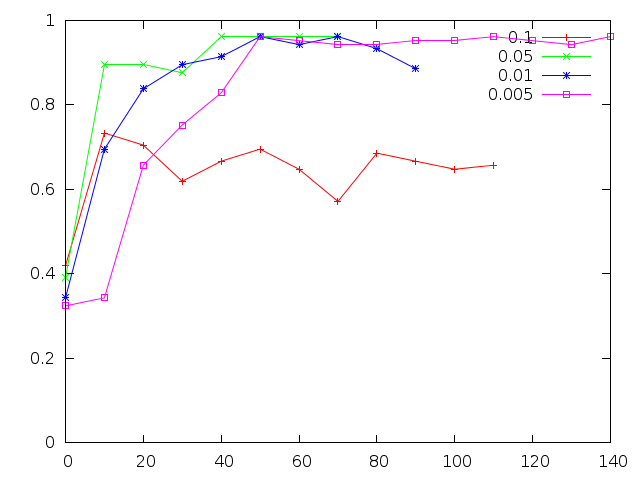
\includegraphics[width=1.0\textwidth]{iris-learningrate-training}
        \caption{Training set acuracy over time with differnt learning rates using the iris dataset.}
        \label{fig:iris_learningrate_training}
    \end{minipage}
    \quad
    \begin{minipage}[b]{0.45\linewidth}
        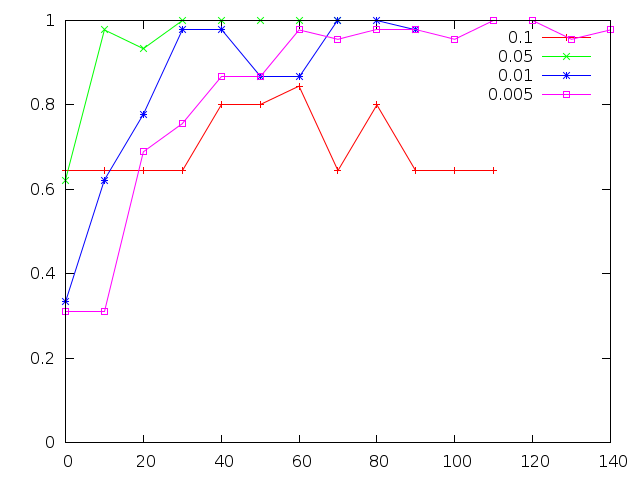
\includegraphics[width=1.0\textwidth]{iris-learningrate-testing}
        \caption{Testing set accuracy over time with different learning rates using the iris dataset.}
        \label{fig:iris_learningrate_testing}
    \end{minipage}
\end{figure}


It seems the best learning rate for iris is $0.05$.

\begin{figure}[!ht]
    \centering
    \begin{minipage}[b]{0.45\linewidth}
        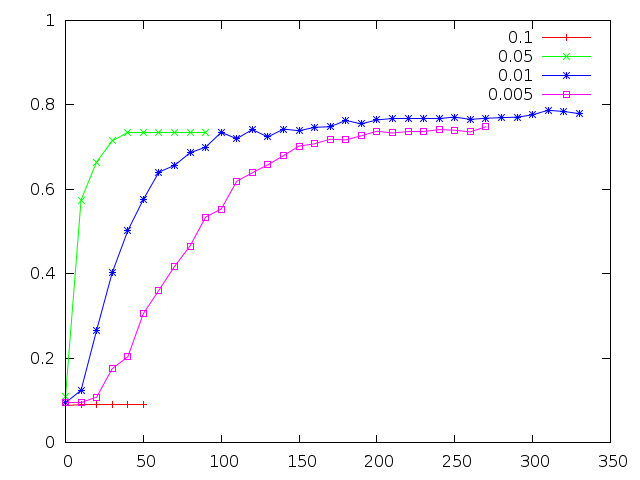
\includegraphics[width=1.0\textwidth]{vowel-learningrate-training}
        \caption{Training set acuracy over time with differnt learning rates using the vowel dataset.}
        \label{fig:vowel_learningrate_training}
    \end{minipage}
    \quad
    \begin{minipage}[b]{0.45\linewidth}
        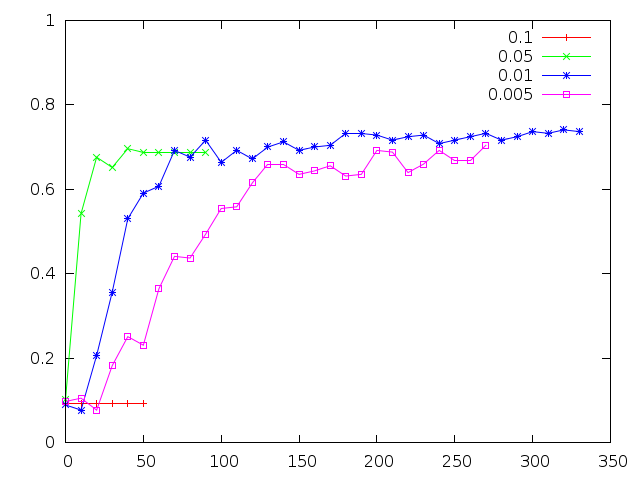
\includegraphics[width=1.0\textwidth]{vowel-learningrate-testing}
        \caption{Testing set accuracy over time with different learning rates using the vowel dataset.}
        \label{fig:vowel_learningrate_testing}
    \end{minipage}
\end{figure}

Doing the same experiment with the vowel dataset, using a single layer of 8
hidden nodes, we find that the best learning rate for vowel is $0.01$. See
figures \ref{fig:vowel_learningrate_training} and \ref{fig:vowel_learningrate_testing}.

\section{Hidden Nodes}
Running various experiments with the iris dataset, using a learning rate of
$0.05$, it seems that with each node,
accuracy improves greatly. It seems that only $3$ nodes are needed to produce
optimal results. See figures
\ref{fig:iris_hiddennodes_training} and \ref{fig:iris_hiddennodes_testing}.
\begin{figure}[!ht]
    \centering
    \begin{minipage}[b]{0.45\linewidth}
        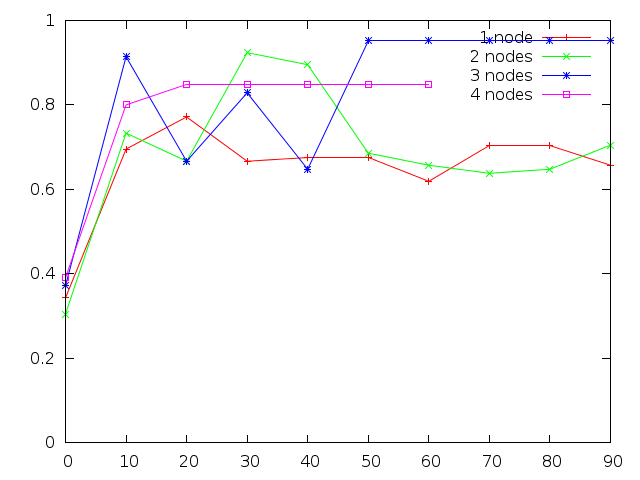
\includegraphics[width=1.0\textwidth]{iris-hiddennodes-training}
        \caption{Training set acuracy over time with differnt sizes of hidden layers using the iris dataset.}
        \label{fig:iris_hiddennodes_training}
    \end{minipage}
    \quad
    \begin{minipage}[b]{0.45\linewidth}
        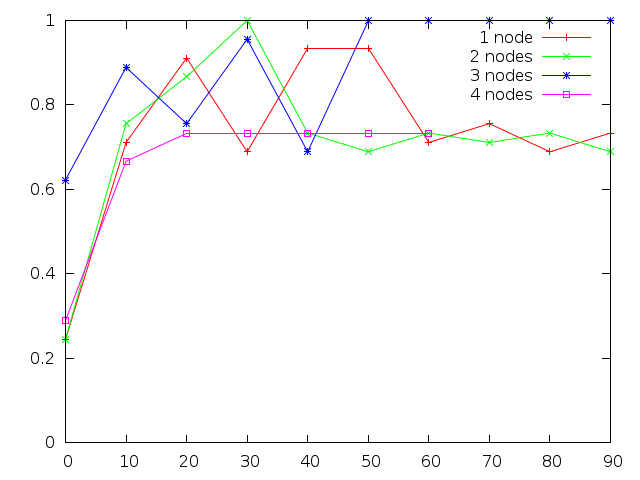
\includegraphics[width=1.0\textwidth]{iris-hiddennodes-testing}
        \caption{Testing set accuracy over time with different sizes of hidden layers using the iris dataset.}
        \label{fig:iris_hiddennodes_testing}
    \end{minipage}
\end{figure}

Repeating the experiments with the vowel dataset, with the learning rate as
$0.01$, we find that it takes more nodes to get the same results. Incrementing
the size of the middle layer node-by-node, The accuracy started to plateu
around $10$ nodes. See figures \ref{fig:vowel_hiddennodes_training} and \ref{fig:vowel_hiddennodes_testing}.

\begin{figure}[!ht]
    \centering
    \begin{minipage}[b]{0.45\linewidth}
        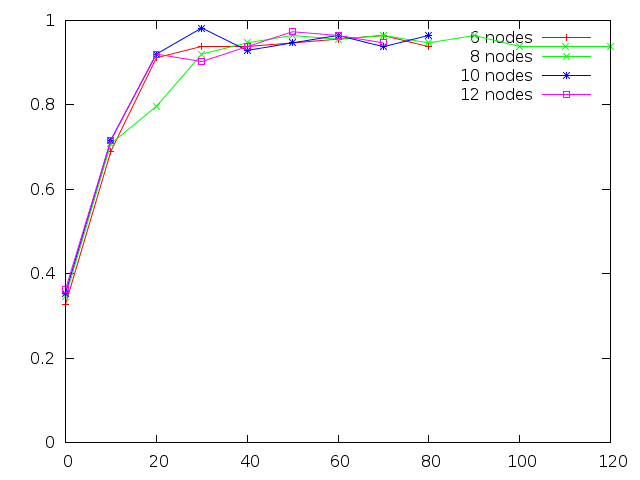
\includegraphics[width=1.0\textwidth]{vowel-hiddennodes-training}
        \caption{Training set acuracy over time with differnt sizes of hidden layers using the iris dataset.}
        \label{fig:vowel_hiddennodes_training}
    \end{minipage}
    \quad
    \begin{minipage}[b]{0.45\linewidth}
        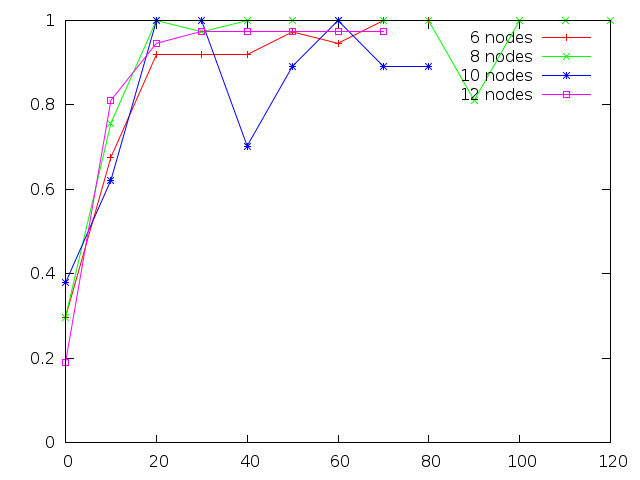
\includegraphics[width=1.0\textwidth]{vowel-hiddennodes-testing}
        \caption{Testing set accuracy over time with different sizes of hidden layers using the iris dataset.}
        \label{fig:vowel_hiddennodes_testing}
    \end{minipage}
\end{figure}
\section{Vowel Dual-Layer Experiment}
Per the project specs, I experimented with two hidden layers on the vowel set,
the first with 6 nodes, and the second hidden layers with 4 nodes, using a
learning rate of $0.01$. Interestingly, the first time I did this, the
accuracy hit a plateu quickly, and did very poorly. I had to reset the random
seed for this experiment, after which the algorithm did very well, as is
summarized in figures \ref{fig:vowel_special_training} and
\ref{fig:vowel_special_testing}.
\begin{figure}[!ht]
    \centering
    \begin{minipage}[b]{0.45\linewidth}
        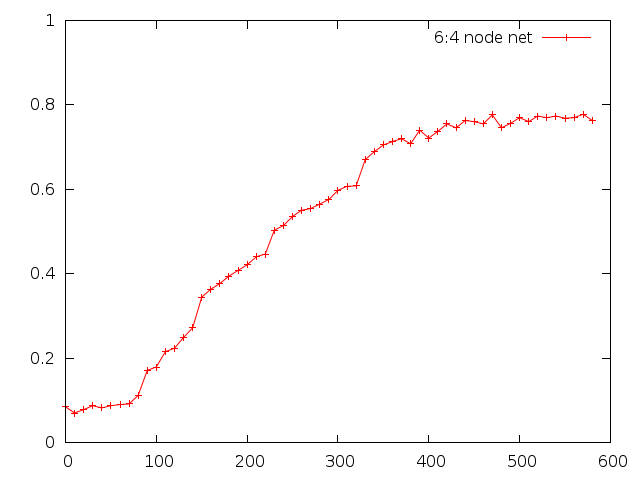
\includegraphics[width=1.0\textwidth]{vowel-special-training}
        \caption{Training set acuracy over time for the vowel 4-6 experiment.}
        \label{fig:vowel_special_training}
    \end{minipage}
    \quad
    \begin{minipage}[b]{0.45\linewidth}
        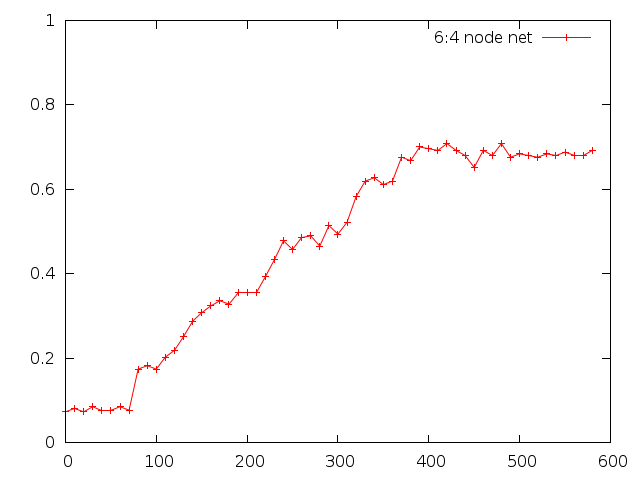
\includegraphics[width=1.0\textwidth]{vowel-special-testing}
        \caption{Testing set accuracy over time for the vowel 4-6 experiment.}
        \label{fig:vowel_special_testing}
    \end{minipage}
\end{figure}
\section{Momentum}
Looking at momentum terms, I simply tried 5 different learning rates for each
dataset (iris and vowel): $0.1$, $0.2$, $0.3$, $0.4$, and $0.5$, depicted in
figures \ref{fig:iris_momentum_training},
\ref{fig:iris_momentum_testing},
\ref{fig:vowel_momentum_training}, and
\ref{fig:vowel_momentum_testing}. For the dataset, we use the learning rate of
$0.05$ and we use $0.01$ for the vowel dataset. As to number of nodes in the
hidden layer of nodes, we use $3$ nodes on the iris dataset experiments, and for
the vowel dataset experiments, we use $10$.
Looking at the graphs, it seems that $0.3$ as the momentum yields the most
return, although $0.4$ still worked pretty well.
\begin{figure}[!ht]
    \centering
    \begin{minipage}[b]{0.45\linewidth}
        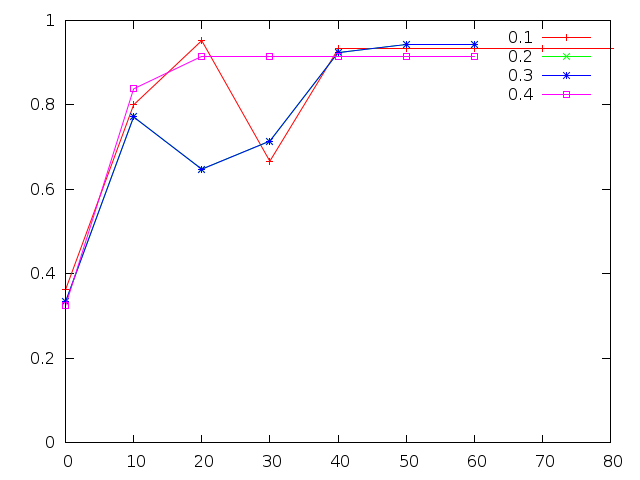
\includegraphics[width=1.0\textwidth]{iris-momentum-training}
        \caption{Training set acuracy over time with different momentum weights for the iris dataset.}
        \label{fig:iris_momentum_training}
    \end{minipage}
    \quad
    \begin{minipage}[b]{0.45\linewidth}
        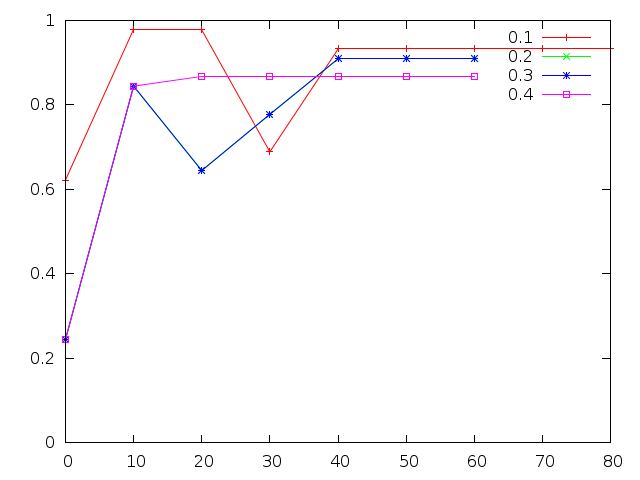
\includegraphics[width=1.0\textwidth]{iris-momentum-testing}
        \caption{Testing set acuracy over time with different momentum weights for the iris dataset.}
        \label{fig:iris_momentum_testing}
    \end{minipage}
\end{figure}
\begin{figure}[!ht]
    \centering
    \begin{minipage}[b]{0.45\linewidth}
        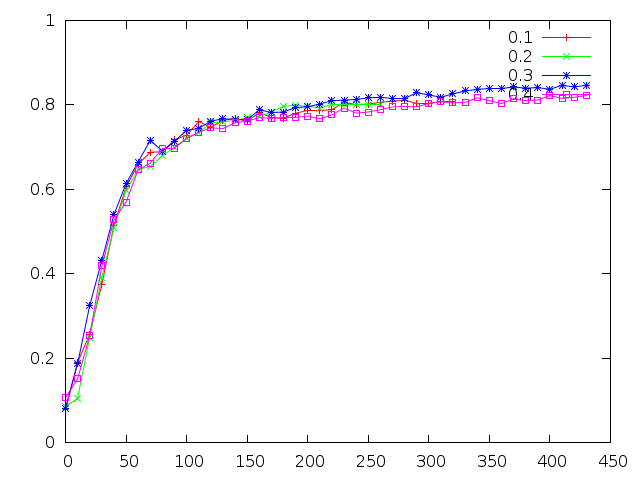
\includegraphics[width=1.0\textwidth]{vowel-momentum-training}
        \caption{Training set acuracy over time with different momentum weights for the vowel dataset.}
        \label{fig:vowel_momentum_training}
    \end{minipage}
    \quad
    \begin{minipage}[b]{0.45\linewidth}
        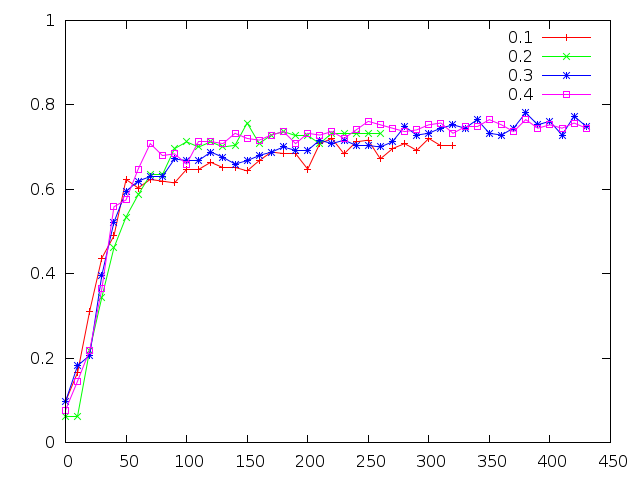
\includegraphics[width=1.0\textwidth]{vowel-momentum-testing}
        \caption{Testing set acuracy over time with different momentum weights for the vowel dataset.}
        \label{fig:vowel_momentum_testing}
    \end{minipage}
\end{figure}

\end{document}
